%chktex-file 1 %chktex-file 2 %chktex-file 3 %chktex-file 8 %chktex-file 9 %chktex-file 10 %chktex-file 11 %chktex-file 12 %chktex-file 13 %chktex-file 16 %chktex-file 17 %chktex-file 18 %chktex-file 25 %chktex-file 26 %chktex-file 35 %chktex-file 36 %chktex-file 37 %chktex-file 40 %chktex-file 44 %chktex-file 45 %chktex-file 49
\section{Евклидовы пространства и их обобщения}
\subsection{Основные понятия и утверждения}
Основное поле - $\F = \R$.
\begin{definition}
    Вещественное конечномерное векторное пространство $\mathcal{E}$ называется евклидовым, если на $\mathcal{E}$ задано скалярное произведение $(x,y)$.
\end{definition}
\begin{definition}
    Скалярное произведение $(x,y)$ - симметрическая билинейная функция такая, что соответственная квадратичная форма $(x,x)$ положительно определена.
\end{definition} 
\begin{definition}
    Длина (норма) вектора $x\in\mathcal{E}$: $|x| = \sqrt{(x,x)}$.
\end{definition}
\begin{theorem} \textbf{Неравенство Коши-Буняковского-Шварца}\\
    $\forall \ x,y\in\mathcal{E}: \ |(x,y)|\leqslant|x|\cdot|y|$, причём равенство выполнено $\Longleftrightarrow  x \parallel y$ (либо $x = 0$ или $y = 0$, либо $y = \lambda x$).
\end{theorem}
\begin{proof}
    Рассмотрим функцию: 
    $$f(t) = (tx-y, tx-y) = t^2(x,x) -2t(x,y) + (y,y) \geqslant 0$$
    Это квадратичная функция относительно $t$:
    $$f(t)\geqslant 0 \Longleftrightarrow  \frac{\mathcal{D}}{4} = (x,y)^2 - (x,x)(y,y) \leqslant 0 \Longrightarrow  (x,y) \leq \sqrt{(x,x)(y,y)} = |x|\cdot|y|$$
    Равенство выполнено $\Longleftrightarrow  (tx-y, tx-y) = 0 \Longrightarrow  y = tx$.
\end{proof}
\begin{theorem} \textbf{Неравенство треугольника}\\
    $\forall x, y \in \mathcal{E} : \ |x+y| \leq |x| + |y|$ \ (равенство выполнено $\Longleftrightarrow x \uparrow \uparrow y$ ) 
\end{theorem}
\begin{proof}
    $$(x+y, x+y) = (x, x) + 2(x, y) + (y, y) \leq |x|^2 + 2|x||y| + |y|^2 = (|x|+|y|)^2$$
    $$|x+y|^2 \leqslant (|x|+|y|)^2 \Longleftrightarrow |x+y| \leq |x| + |y|$$  
\end{proof}
Координатная запись: пусть в $V$ фиксированный базис $e_1,...,e_n$, то: 
$$(x,y) = (\sum \limits_{i=1}^nx_ie_i, \sum \limits_{j=1}^ny_je_j) = \sum \limits_{i,j=1}^nx_iy_j(e_i,e_j)$$
\begin{definition}
    $G_e = ((e_i,e_j))$ - матрица Грама базиса $e$
    $$G_e^T = G_e$$ 
    Т.к. $(x,x)$ - положительно определенная квадратичная форма, то матрица: 
    $$G_e = (g_{ij})$$ 
    может служить матрицей Грама $\Longleftrightarrow \triangle_1 >0,...,\triangle_n > 0$ \\
    В частности: \ $\det G_e >0$ (определитель Грама)   
\end{definition}
\begin{center}
    \fbox{\text{ $(x,y) = X^TG_eY$ }}
\end{center}
\begin{definition}
    $$x \perp y \Longleftrightarrow (x,y) = 0$$ 
\end{definition}
\begin{definition}
    Базис $e_1,...,e_n$ называется ортогональным, если: 
    $$e_i \perp e_j \ \text{ при } i \neq j$$
    Ecли при этом длина каждого вектора $e_1,...,e_n$ равна 1, то базис называется ортонормированным.
\end{definition}
\begin{consequense}
    $e_1,...,e_n$ - ортонормированный базис, если $(e_i,e_j) = \delta_{ij}$.  
\end{consequense}
\begin{consequense}
    Если базис ортонормированный, то $G = E$ и $(x,y) = \sum \limits_{i=1}^nx_iy_i$.
\end{consequense}
\begin{theorem} Пусть $e' = eC_{e\to e'}$ - новый базис. Тогда: 
    \begin{enumerate}
        \item Если $e$ и $e'$ - ортонормированные базисы, то $C_{e \to e'}$ ортогональна;
        \item Если $e$ - ортонормированный базис и $C_{e \to e'}$ ортогональная матрица $\Longrightarrow e' = eC$ - ортонормированный базис.
    \end{enumerate}
\end{theorem}
\begin{remark}
    $C$ - ортогональная, если $C^TC = E$  
\end{remark} 
\begin{proof} \tab
    \begin{enumerate}
        \item По определению матрицы перехода:
        $$C_{e \to e'} = \begin{pmatrix}
            e_1'^{\uparrow} & \cdots & e_n'^{\uparrow}
        \end{pmatrix}; \ \ 
        C^T_{e\to e'} = \begin{pmatrix}
            e_1'^{\rightarrow}  \\ \vdots \\ e_n'^{\rightarrow} 
        \end{pmatrix}$$ 
        Обозначим $d_{ij}$ - $(ij)$ элемент матрицы $C^TC:$ 
        $$d_{ij} = e_i'^{\rightarrow} \cdot e_j'^{\uparrow} = (e'_i,e_j') = \delta_{ij}$$
        т.к. базис $e$ ортонормированный $\Longrightarrow d_{ij} = \delta_{ij} \Longrightarrow C^TC = E$
        \item Рассмотрим $e' = eC_{e\to e'}$, тогда $e_j^{\uparrow}$ - это $j$ столбец матрицы $C_{e\to e'}$\\
        По условию $C^TC = E \Longleftrightarrow e_i'^{\rightarrow} \cdot e_j'^{\uparrow} = \delta_{ij} = (e'_i,e_j')$
    \end{enumerate}    
\end{proof}
\begin{lemma}
    Если $a_1,...,a_m \in \mathcal{E}$ - ортогональная система векторов, то $a_1,...,a_m$ ЛНЗ. 
\end{lemma}
\begin{proof}
    Пусть $\sum \limits_{i=1}^m \lambda_ia_i = 0$. Скалярно умножим обе части на $a_j$:
    \[(\sum \limits_{i=1}^m \lambda_ia_i, a_j) = \sum \limits_{i=1}^m \lambda_i(a_i, a_j) = \lambda_j(a_j, a_j) = 0 \Longrightarrow \lambda_j = 0\]
    Проведя такие рассуждения для $j = 1,...,m$, получим, что все коэффициенты должны быть равны 0, т.е. $a_1,...,a_m$ ЛНЗ.
\end{proof}
Т.о. $\forall x \in \mathcal{E}$ единственным образом разлагается в сумму $x = x_{\shortparallel} + x_{\perp}$
\begin{center}
    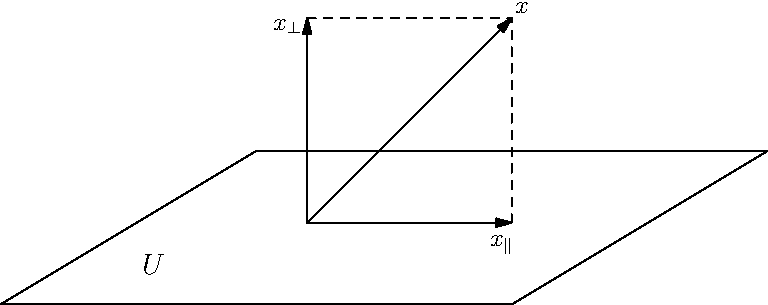
\includegraphics[width=10cm]{image/Asymptote/3/linal-3-1.pdf}
\end{center}
$x_{\shortparallel} \in U, \ \ x_{\shortparallel}$ - ортогональная проекция вектора $x$ на $U$\\
$x_{\perp} \in U^{\perp}, \ x_{\perp}$ - ортогональная составляющая $x$ относительно $U$
\begin{example1}\tab
    \begin{center}
        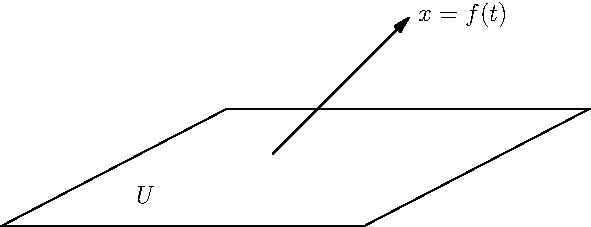
\includegraphics[width=8cm]{image/Asymptote/4/linal-4-1.pdf}
        $U = \langle 1,t,...,t^{n-1} \rangle$ 
    \end{center}
    Надо подобрать такой многочлен $p(t) \in U$, чтобы: 
    $$\parallel f(t) - p(t)\parallel \ = \min$$
    Где $p(t) = f(t)$ - псевдорешение  
\end{example1}
\subsection*{Как конкретно находить такое разложение?}
\begin{itemize}
    \item[\textbf{1 способ:}] Выбрать ортогональный базис в $U$ и дополнить его до ортогонального базиса в $\mathcal{E}$\\
    Тогда:
    $$x = \underbrace{\sum \limits_{i=1}^m(x_i,e_i)e_i}_{x_\shortparallel}  + \underbrace{\sum \limits_{i=m+1}^n(x_i,e_i)e_i}_{x_\perp} = x_\shortparallel + x_\perp$$
    \item[\textbf{2 способ:}] Выбрать в $U$ произвольный базис $a_1,...,a_m$ и искать разложение в виде:
    $$x = \sum \limits_{i=1}^m \alpha_ia_i + x_\perp \ \ | \cdot a_j \Longrightarrow (x_i,a_j) = \sum \limits_{i=1}^m \alpha_i(a_i,a_j) + \underbrace{(x_\perp, a_j)}_{=0} $$
    Неоднородная СЛУ с неизвестными $\alpha_i$, основная матрица: 
    $$((a_i,a_j)) = G_{\{a_1,...,a_m\}}$$
    где $\det G \neq 0 \Longrightarrow$ по теореме Крамера $\exists ! \ \alpha_1,...,\alpha_m \Longrightarrow \exists ! \ x_\shortparallel \Longrightarrow x_\perp = x - x_\shortparallel$   
\end{itemize}
\begin{definition}
    Ортогональное дополнение подпространства $U \subset \E$ - ортогональное дополнение $U$ относительно скалярного произведения как симметрической билинейной формы.
\end{definition}
\begin{remark}
    Доказательство разложения $\E = U \oplus U^\perp$ см. в разделе \ref{oplus}
\end{remark}
\begin{properties} \textbf{операций ортогонального дополнения} 
    \begin{enumerate}
        \item $(U^\perp)^\perp = U$
        \item $(U_1 + U_2)^\perp = U_1^\perp \cap U_2^\perp$
        \item $(U_1 \cap U_2)^\perp = U_1^\perp + U_2^\perp$
    \end{enumerate}
\end{properties}
\begin{proof}\tab
    \begin{enumerate}
        \item Пусть $x\in U,\ y\in U^\perp$, тогда: 
        $$\forall y\in U^\perp: \ (y,x)=0 \Longrightarrow  x\in (U^\perp)^\perp \Longrightarrow  U\subseteq (U^\perp)^\perp$$ 
        Причем: 
        $$\dim{(U^\perp)^\perp}=n-\dim{U^\perp}=n-(n-\dim{U})=\dim{U}\Longrightarrow  U=(U^\perp)^\perp$$

        \item Пусть $v\in U_1^\perp\cap U_2^\perp \Longrightarrow  v\perp U_1$ и $v\perp U_2 \Longrightarrow  \forall x=u_1+u_2$:
        $$(v,x)=(v,u_1)+(v,u_2)=0 \Longrightarrow  v\in (U_1+U_2)^\perp \Longrightarrow  U_1^\perp \cap U_2^\perp \subseteq (U_1+U_2)^\perp$$
        Если $w\in (U_1+U_2)^\perp$, то $\forall u_1\in U_1, \forall u_2\in U_2 :\ (w, u_1+u_2)=0$\\
        В частности: 
        $$\begin{cases}
            \forall u_1\in U_1: \ (w, u_1)=0 \ \Longrightarrow  w\in U_1^\perp\\
            \forall u_2\in U_2: \ (w, u_2)=0 \ \Longrightarrow  w\in U_2^\perp
        \end{cases} \Longrightarrow  w\in U_1^\perp\cap U_2^\perp$$
        То есть $(U_1+U_2)^\perp \subseteq U_1^\perp \cap U_2^\perp \Longrightarrow $ имеет место равенство:
        $$(U_1+U_2)^\perp=U_1^\perp\cap U_2^\perp$$

        \item Возьмем $(U_1^\perp+U_2^\perp)^\perp=(U_1^\perp)^\perp \cap (U_2^\perp)^\perp=U_1 \cap U_2$
        $$\Longrightarrow  ((U_1^\perp+U_2^\perp)^\perp)^\perp=(U_1\cap U_2)^\perp \Longrightarrow  U_1^\perp+U_2^\perp=(U_1 \cap U_2)^\perp$$
    \end{enumerate}
\end{proof}
\begin{subtheorem}
    Вектор наименьшей длины, соединяющий точку из подпространства $U$ с концом вектора $x$ - $x_{\perp}$. 
\end{subtheorem}
\begin{proof}
    Обозначим $x_{\shortparallel} = y, \ x_{\perp} = z$, а вектор из начала $x$ в произвольную точку $U$ - вектор $v$
    \begin{center}
        % 
        Какой тут рисунок то? ( рисунок скинули, завтра нарисую )
    \end{center}
    Докажем, что $|x-v|\geqslant |z|$, причём равенство достигается при $v = y$:
    $$x - v = x - y + y - v = z + y - v$$
    Т.к. $z \in U^{\perp}, (y - v) \in U$,
    $$z \perp (y-v) \Longrightarrow |x-v|^2 = |z|^2 + |y-v|^2 \geqslant |z|^2$$
    причём равенство при $|y - v| = 0 \Longrightarrow y = v$.
\end{proof}
Это подтверждает осмысленность определения $\rho(x, U) = |x_{\perp}|$.
\begin{exercise}
    Докажите отсюда, что $\angle(x, v) \geqslant \angle(x, y)$.
\end{exercise}
\begin{definition}
    Углом между вектором и подпространством будем называть: 
    $$\angle(x, U) = \angle(x, y)$$
\end{definition}

Частный случай: $\dim U = n-1$ ("гиперплоскость"):\\
В ортонормированном базисе $U$ задаётся уравнением $a_1x_1 +...+a_nx_n = 0$, а ортогональное дополнение $U^{\perp} = \langle n = (a_1,...,a_n)\rangle$ ($n$ - вектор нормали). Тогда:
$$\rho(x, U) = |x_{\perp}| = \frac{V_{\langle e_1,...,e_{n-1},x\rangle}}{V_{\langle e_1,...,e_{n-1}\rangle}}$$
где $V_{\langle a_1,...,a_k\rangle}$ - объём параллелепипеда, натянутого на $a_1,...,a_k$.
\begin{definition}
    $n$-мерным параллелепипедом с рёбрами $e_1,...,e_n$ называется:
    $$\Pi_{\langle e_1,...,e_n\rangle} = \{v = \lambda_1e_1 + ... + \lambda_{n}e_{n}, 0\leqslant\lambda_i\leqslant1\}$$
\end{definition}
\begin{definition}
    В общем случае объём параллелепипеда определяется рекурсивно:
    $$V_{\langle e_1,...,e_n\rangle} = V_{\langle e_1,...,e_{n-1}\rangle} \cdot |e_{n\perp}|,  \ \text{где $e_{n\perp}$ - проекция $e_n$ на $\langle e_1,...,e_{n-1}\rangle$}$$
    Заметим, что если $e_1,...,e_n$ попарно ортогональны, то $V_{\langle e_1,...,e_n\rangle} = |e_1|\cdot...\cdot|e_n|$.
\end{definition}
Объём не изменится, если к векторам применить процесс ортогонализации (с унитреугольной матрицей перехода).\\
Тогда: 
$$V_{\langle e'_1,...,e'_n\rangle} = |e'_1|\cdot...\cdot|e'_n| = \sqrt{|G_{\{ e'_1,...,e'_n\}}|}$$
В ортогональном базисе: 
$$G_{\{ e'_1,...,e'_n\}} = \begin{pmatrix} |e'_1|^2 &\null&0 \\ \null&\ddots&\null \\ 0&\null&|e'_n|^2 \end{pmatrix} \Longrightarrow  |G_{\{ e'_1,...,e'_n\}}| = |e'_1|^2\cdot...\cdot|e'_n|^2$$
$$G_{e'} = C^TG_eC \Longrightarrow |G_{e'}| = |C|^2|G_e| = |G_e|$$
\begin{exercise}
    Доказать отсюда. что если $U = \langle e_1,...,e_{n-1}\rangle$, то:
    $$\rho^2(x, U) = \frac{|G_{\{ e_1,...,e_n\}}|}{|G_{\{ e_1,...,e_{n-1}\}}|}$$
\end{exercise}
\subsection{Линейные операторы в евклидовом пространстве}
Пусть $\mathcal{E}$ - евклидово пр-во, $\phi: \mathcal{E} \rightarrow \mathcal{E}$ - лин. оператор в $\mathcal{E}$.
\begin{definition} \tab
    \begin{enumerate}
        \item Оператор $\phi^{*}: \mathcal{E} \rightarrow \mathcal{E}$ - сопряжённый к $\phi$, если:
        $$\forall x,y \in \mathcal{E}: \ (\phi(x), y) = (x, \phi^{*}(y)) \eqno{(1)}$$
        \item Оператор $\phi$ - самосопряжённый, если:
        $$\phi^{*} = \phi \Longrightarrow \forall x,y \in \mathcal{E}: \ (\phi(x), y) = (x, \phi(y)) \eqno{(2)}$$
        \item Оператор $\phi$ - ортогональный, если:
        $$\forall x,y \in \mathcal{E}: \ (\phi(x), \phi(y)) = (x, y) \eqno{(3)}$$
        В частности, для ортогонального $\phi: \forall x \in \mathcal{E} \ \ |\phi(x)| = |x|$.
    \end{enumerate}
\end{definition}
\textbf{Условия (1)-(3) через матрицу Грама}\\
    Пусть в $\mathcal{E}$ зафиксирован базис $e = (e_1,...,e_n) \ (\dim \mathcal{E} = n)$. Пусть $x = eX,\\
    y = eY, G_e = ((e_i, e_j))$ - матрица Грама базиса $e$, $A_{\phi}$ - матрица $\phi$ в базисе $e$.\\
    (1): $\forall X, Y \in \R^n$:
    $$(A_{\phi}X)^TG_eY = X^TA_{\phi}^TG_eY = X^TG_eA_{\phi^{*}}Y \Longrightarrow A_{\phi}^TG_e = G_eA_{\phi^{*}} \ \ (1')$$
    (2): В частности, 
    $$\phi^{*} = \phi \Longleftrightarrow  A_{\phi}^TG_e = G_eA_{\phi} (2')$$
    Если $e$ - ортонормированный, то $G_e = E$, и $A_{\phi}^T = A_{\phi}$, т.е. $A_{\phi}$ - симметрическая матрица.\\
    (3): $\phi$ - ортогональный $\Longleftrightarrow  \ \forall X, Y \in \R^n$ выполнено:
    $$(A_{\phi}X)^TG_e(A_{\phi}Y) = X^TG_eY \Longrightarrow A_{\phi}^TG_eA_{\phi} = G_e (3')$$
    Если $G_e = E$, то $A_{\phi}^TA_{\phi} = E$, т.е. $A_{\phi}$ - ортогональная матрица.
\begin{theorem}\textbf{Свойства сопряжённых операторов}
    \begin{enumerate}
        \item $(\phi^{*})^{*} = \phi$;
        \item $\textup{Ker}\phi^{*} = (\textup{Im}\phi)^{\perp}$
        \item $\textup{Ker}\phi = (\textup{Im}\phi^{*})^{\perp}$
    \end{enumerate}    
\end{theorem}
\begin{proof} \tab
    \begin{enumerate}
        \item В ортонормированном базисе:
        $$A_{\phi^{*}} = A_{\phi}^T \Longrightarrow  A_{{\phi^{*}}^{*}} = (A_{\phi^{*}})^T = (A_{\phi}^T)^T = A_{\phi}$$
        Т.к. в фиксированном базисе имеется взаимно однозначное соответствие операторов и их матриц, $(\phi^{*})^{*} = \phi$.
        \item Сравним размерности:
        $$\dim \textup{Ker}\phi^{*} = n - \textup{rk}(A_{\phi^{*}}) = n - \textup{rk}(A_{\phi}^T) = n - \textup{rk}(A_{\phi})$$
        $$\dim \textup{Im}\phi = \textup{rk} A_{\phi} \Longrightarrow \dim (\textup{Im}\phi)^{\perp} = \textup n - {rk} A_{\phi}$$
        Докажем, что $\textup{Im}\phi \subseteq (\textup{Ker}\phi^{*})^{\perp}$  (отсюда $\textup{Ker}\phi^{*} \subseteq (\textup{Im}\phi)^{\perp}$):\\
        Пусть $v \in \textup{Im}\phi \Longrightarrow v = \phi(x)$, $y \in \textup{Ker}\phi^{*}$. Тогда:
        $$(v, y) = (\phi(x), y) = (x, \phi^{*}(y)) = (x, 0) = 0 \Longrightarrow v \perp \textup{Ker}\phi^{*}$$
        Т.к. размерности равны и $\textup{Ker}\phi^{*} \subseteq (\textup{Im}\phi)^{\perp}$, то $\textup{Ker}\phi^{*} = (\textup{Im}\phi)^{\perp}$.
        \item Следует из (2) подстановкой $\phi^{*}$ вместо $\phi$.
    \end{enumerate}
\end{proof}
\begin{consequense}\textbf{Теорема Фредгольма}
    СЛУ $AX = b$ с квадратной матрицей $A$ порядка $n$ совместна $\Longleftrightarrow $ для любого $Y$ - решения однородной сопряжённой системы - выполнено условие $Y \perp b$. 
\end{consequense}
\begin{proof}
    $AX = b$ совместна $\Longleftrightarrow  b \in \textup{Im}A$
    $$Y \in \textup{Ker}\phi^{*} = \textup{Ker}A^T$$
    Т.к. $\textup{Ker}\phi^{*} = (\textup{Im}A)^\perp$, то система совместна $\Longleftrightarrow  b \perp \textup{Ker}\phi^{*}$  
\end{proof}
\subsection{Самосопряжённые операторы}
\begin{lemma}
    Пусть $\phi: \E \rightarrow \E$ - лин. оператор, $U \subset \E: \phi(U) \subseteq U$.\\
    Тогда $\phi^*(U^\perp) \subseteq U^\perp$.
\end{lemma}
\begin{proof}
    Покажем, что $\forall y \in U^\perp, x \in U$ выполнено $(x, \phi^*(y)) = 0$:
    $$(x, \phi^*(y)) = (\phi(x), y) = 0, \text{ т.к. } \phi(x) \in U, \ y \in U^\perp$$
\end{proof}
\begin{subtheorem} \tab
    \begin{enumerate}
        \item Если $\lambda_1, \lambda_2$ - различные собственные значения самосопряжённого оператора $\phi$, $x_1, x_2$ - соответсвующие им собственные векторы, то $x_1 \perp x_2$;
        \item Все характеристические числа самосопряжённого оператора $\in \R$.
    \end{enumerate}
\end{subtheorem}
\begin{proof} \tab
    \begin{enumerate}
        \item Пусть $\phi^* = \phi$. Тогда:
        $$(\phi(x_1), x_2) = \lambda_1(x_1, x_2); \ (\phi(x_1), x_2) = (x_1, \phi(x_2)) = \lambda_2(x_1, x_2)$$
        Из $\lambda_1 \neq \lambda_2$ следует $(x_1, x_2) = 0$. 
        \item От противного: пусть $\exists \lambda_1 = \alpha + i\beta$ - характеристическое число для самосопряжённого $\phi$ с $\beta \neq 0$.\\
        Как было доказано ранее, $\exists \ \phi$-инвариантное подпространство $U$ размерности 2, на котором $\phi|_U$ имеет собственные значения $\alpha \pm i\beta$.
        $U$ можно рассматривать как евклидово пр-во со скалярным произведением $(x, y)|_U$. Тогда $\phi|_U$ - также самосопряжённый на $U$.\\
        Выберем ортонормированный базис в $U$. Тогда в этом базисе $\phi|_U$ имеет симметрическую матрицу $A = \begin{pmatrix} a_{11}&a_{12} \\ a_{12}&a_{22} \end{pmatrix}$. Её характеристические числа:
        $$|A - \lambda E| = (a_{11} - \lambda)(a_{22} - \lambda) - a_{12}^2 = \lambda^2 - (a_{11} + a_{22})\lambda + a_{11}a_{22} - a_{12}^2$$
        $$\mathcal{D} = (a_{11} + a_{22})^2 - 4a_{11}a_{22} + 4a_{12}^2 = (a_{11} - a_{22})^2 + 4a_{12}^2 \geqslant 0$$
        Отсюда корни характеристического многочлена вещественные, что противоречит предположению.
    \end{enumerate}
\end{proof}
\begin{theorem}
    Для любого самосопряжённого оператора $\phi: \mathcal{E} \rightarrow \mathcal{E}$ в $\mathcal{E}$ существует ортонормированный базис из собственных векторов этого оператора.
\end{theorem}
\begin{proof}
    Индукция по $\dim \E = n$:\\
    База: $n = 1$. Тогда $\forall x \in \E: \ \phi(x) = \lambda_1 x$, т.е. любой вектор длины 1 подойдёт в качестве ортонормированного базиса.\\
    Шаг: Пусть $\lambda_1 \in \R$ - какое-либо собственное значение для $\phi$. Рассмотрим $\E_{\lambda_1} \neq \{0\}$ - оно является $\phi$-инвариантным подпространством.\\
    Если $\E_{\lambda_1} = \E$, то $\forall x \in \E: \ \phi(x) = \lambda_1 x$, т.е. в ортонормированном базисе матрица оператора - $\lambda_1 E$;\\
    Если $\E_{\lambda_1} \neq \E$, то по лемме $\E_{\lambda_1}^\perp$ также $\phi$-инвариантно и $\E = \E_{\lambda_1} \oplus \E_{\lambda_1}^\perp$. К ограничению $\phi$ на инвариантные подпространства $\E_{\lambda_1}, \E_{\lambda_1}^\perp$ можно применить предположение индукции, если рассмотреть их как отдельные евклидовы пространства. Тогда в них есть ортонормированные базисы из собственных векторов, а тогда их объединение будет искомым ортонормированным базисом для $\E$ (ортогональность векторов из разных базисов следует из утверждения выше).
\end{proof}
\begin{consequense}
    Если $\lambda_1,...,\lambda_s$ - все попарно различные собственные значения самосопряжённого оператора $\phi$, то $\E = \E_{\lambda_1} \oplus ... \oplus \E_{\lambda_s}$.
\end{consequense}
\begin{remark}
    Если все собственные значения $\lambda_1,...,\lambda_n$ самосопряжённого оператора $\phi$ положительны, то $\exists$ самосопряжённый оператор $\psi$ с положительными собственными значениями такой, что $\psi^2 = \phi$.
\end{remark}
\begin{proof}
    Пусть $e_1,...,e_n$ - ортонормированный базис из собственных векторов для $\phi$. Тогда: 
    $$A_{\phi, e} = \begin{pmatrix} \lambda_1&\null&\null \\ \null&\ddots&\null \\ \null&\null&\lambda_n \end{pmatrix} \Longrightarrow \text{ оператор с матрицей } \begin{pmatrix} \sqrt{\lambda_1}&\null&\null \\ \null&\ddots&\null \\ \null&\null&\sqrt{\lambda_n} \end{pmatrix} - \psi$$
\end{proof}
\begin{example1}
    Пусть $\E = U \oplus U^\perp$, т.е. $\forall x = x_\shortparallel + x_\perp$.\\
    $\phi_1(x) = x_\shortparallel$ - ортогональное проектирование на $U$;\\
    $\phi_2(x) = x_\shortparallel - x_\perp$ - ортогональная симметрия, или отражение $\E$ относительно $U$.\\
    Покажем, что $\phi_1$ и $\phi_2$ самосопряжённые:
    $$\forall x,y \in \E: x = x_\shortparallel + x_\perp, y = y_\shortparallel + y_\perp :$$
    $$(\phi_1(x), y) = (x_\shortparallel, y_\shortparallel + y_\perp) = (x_\shortparallel, y_\shortparallel) = (x_\shortparallel + x_\perp, y_\shortparallel) = (x, \phi_1(y))$$
    $$(\phi_2(x), y) = (x_\shortparallel - x_\perp, y_\shortparallel + y_\perp) = (x_\shortparallel, y_\shortparallel) - (x_\perp, y_\perp) = (x_\shortparallel + x_\perp, y_\shortparallel - y_\perp) = (x, \phi_2(y))$$
\end{example1}

\subsection{Ортогональные операторы}
\begin{definition}
    $\phi: \E \rightarrow \E$ - ортогональный, если: 
    $$\forall x,y \in \E: \ (\phi(x), \phi(y)) = (x, y)$$ 
\end{definition}
Из определения следует, что $\forall x \in \E: \ |\phi(x)| = |x|$ - $\phi$ сохраняет длины $\Longrightarrow \textup{Ker}\phi = \{0\} \Longrightarrow \phi$ инъективный, а так как $\phi: \E_n \rightarrow \E_n$, получаем, что $\phi$ - биективный (и обратимый) оператор.  
\begin{subtheorem}
    Пусть $\phi: \E \rightarrow \E$ - ортогональный оператор.\\
    Тогда $\phi^{-1}$ также ортогональный, причём $\phi^{-1} = \phi^*$.
\end{subtheorem}
\begin{proof}
    Покажем, что $\forall x,y \in \E (\phi^{-1}(x), \phi^{-1}(y)) = (x, y)$. Выберем $x' = \phi^{-1}(x), y' = \phi^{-1}(y)$. Тогда:
    $$(\phi^{-1}(x), \phi^{-1}(y)) = (x', y') = (\phi(x'), \phi(y')) = (x, y)$$
    По определению $\phi^*$: $(\phi(x), y) = (x,\phi^*(y)), \ \forall x, y \in \E$\\
    Т.к. $\phi$ обратим, $\exists y' \in E: \ y = \phi(y')$
    $$(\phi(x), y) = (\phi(x), \phi(y')) = (x, y') = (x, \phi^{-1}(y)) \Longrightarrow (x, \phi^*(y)) = (x, \phi^{-1}(y))$$
    $$(x, \phi^*(y) - \phi^{-1}(y)) = 0 \ \forall x,y \in \E \Longrightarrow \phi^*(y) = \phi^{-1}(y) \ \forall y \in \E$$
    т.е. $\phi^* = \phi^{-1}$
\end{proof}
\begin{lemma}
    Пусть $\phi: \E \rightarrow \E$ - ортогональный оператор, $U \subset E: \ \phi(U) \subseteq U$.\\
    Тогда: $$\phi(U^\perp) \subseteq U^\perp$$
\end{lemma}
\begin{proof}
    Покажем, что $\forall y \in U^\perp, x \in U$ выполнено $(x, \phi(y)) = 0$.\\
    Т.к. $\phi$ обратим, $\exists x': x = \phi(x')$, т.е. $x' = \phi^{-1}(x) \in U$. Отсюда:
    $$(x, \phi(y)) = (\phi(x'), \phi(y)) = (x', y) = 0, \text{ т.к. } x' \in U, \ y \in U^\perp$$
\end{proof}
\begin{definition}
    В пространстве $\mathcal{C}^n$ введем скалярное произведение с требованиями:
\begin{enumerate}
    \item Линейность по 1 аргументу
    \item Вместо симметричности потребуем:
    $$(y,x) = \overline{(x,y)}$$
    \item $(x,x) \neq 0, \ (x,x) = 0$, если $x=0$   
\end{enumerate}
Следовательно, если $\lambda \in \CC$, то $(x,\lambda y) = \overline{\lambda}(x,y)$ 
\end{definition}
\begin{theorem}
    Пусть $\phi: \E \rightarrow \E$ - ортогональный оператор.
    \begin{enumerate}
        \item Собственные значения $\phi$ - только $\pm 1$, причём отвечающие этим значениям собственные векторы $\perp$.
        \item Все характеристические числа для $\phi$ над $\mathbb{C}$ имеют модуль 1. 
    \end{enumerate}
\end{theorem}
\begin{proof}\tab
    \begin{enumerate}
        \item Пусть $\phi(x) = \lambda x, x \neq 0, \lambda \in \R$. Тогда:
        $$(x, x) = (\phi(x), \phi(x)) = \lambda^2(x,x) \Longrightarrow \lambda^2 = 1 \Longrightarrow \lambda = \pm 1$$ 
        Если $\phi(x) = x, \phi(y) = -y (x,y \neq 0)$, то
        $$(x, y) = (\phi(x), \phi(y)) = -(x, y) \Longrightarrow (x, y) = 0$$
        \item Будем обозначать через $\phi: \ \CC^n \to \CC^n$ заданной матрицей $A_\phi$ \\
        Если $\lambda = \alpha + i\beta$ - характеристическое число для $\phi$, то: 
        $$\exists \ v \in \CC^n: \ \phi(v) = \lambda(v)$$
        Тогда $(v, v) = (\phi(v), \phi(v)) = (\lambda v, \lambda v) = \lambda \overline{\lambda}(v,v) \Longrightarrow \lambda \overline{\lambda} = |\lambda|^2 = 1$, или $\lambda = \cos(\theta) \pm i \sin(\theta)$.
    \end{enumerate}
\end{proof}
\begin{theorem}
    Если $\phi: \ \E \to \E$ - ортогональный оператор, то в $\E \ \exists$ ортонормированный базис, в котором:
    $$A_{\phi,f} = \begin{pmatrix}
        \text{\fbox{$\Phi_1$}}\\
        \null & \ddots\\
        \null & \null & \text{\fbox{$\Phi_s$}}\\
        \null & \null & \null & \text{\fbox{$1$}} \\
        \null & \null & \null & \null & \ddots \\
        \null & \null & \null & \null & \null & \text{\fbox{$1$}}\\
        \null & \null & \null & \null & \null & \null & \text{\fbox{$-1$}} \\
        \null & \null & \null & \null & \null & \null & \null & \ddots \\
        \null & \null & \null & \null & \null & \null & \null & \null & \text{\fbox{$-1$}}
    \end{pmatrix}, \ \Phi_i = \begin{pmatrix}
        \cos \alpha_i & -\sin \alpha_i \\ \sin \alpha_i & \cos \alpha_i
    \end{pmatrix}$$   
    Порядок матрицы равен $ n = \dim \E$ ($s$ - количество пар сопряжённых собственных значений, а также количество 1 и -1 определены однозначно). 
\end{theorem} 
\begin{proof}
    Заметим, что если все собственные значения $\phi$ вещественные, то для $\phi$ существует ортонормированный базис из собственных векторов - это объединение ортонормированных базисов подпространств $\E_{1}$ и $\E_{-1}$ (в частности, $\phi$ будет ещё и самосопряжённым).\\
    Индукция по $n$:\\
    База: $n = 2$. Случай, если все собственные значения $\phi$ вещественные, разобран. Если у $\phi$ есть комплексное собственное значение $\lambda$, то $\overline{\lambda}$ - также собственное значение для $\phi$. Рассмотрим произвольный ортонормированный базис $e_1, e_2 \in \E$. В нём $\phi(e_1) = \alpha e_1 + \beta e_2$. Так как $\phi$ сохраняет длины, $|\phi(e_1)| = 1$, т.е.
    \[(\alpha e_1 + \beta e_2, \alpha e_1 + \beta e_2) = \alpha^2 + \beta^2 = 1 \Longrightarrow \exists \psi_1: \ \alpha = \cos(\psi_1), \beta = \sin(\psi_1)\]
    Аналогично $\exists \psi_2: \ \phi(e_2) = \cos(\psi_2)e_1 + \sin(\psi_2)e_2$. При этом $(\phi(e_1), \phi(e_2)) = (e_1, e_2) = 0$, т.е.
    \[(\phi(e_1), \phi(e_2)) = \cos\psi_1\cos\psi_2 + \sin\psi_1\sin\psi_2 = \cos(\psi_1 - \psi_2) = 0\] 
    Отсюда $\psi_2 = \psi_1 + \frac{(2k+1)\pi}{2}$, т.е. при необходимости заменив $e_2$ на $-e_2$ в базисе, получим матрицу $A_\phi = \begin{pmatrix} \cos\psi_1 & -\sin\psi_1 \\ \sin\psi_1 & \cos\psi_1 \end{pmatrix}$. База доказана.\\
    Переход: пусть $n > 2$. Случай, если все собственные значения $\phi$ вещественные, разобран. Если у $\phi$ есть комплексное собственное значение $\lambda$, то из доказанного ранее знаем, что существует $\phi$-инвариантное подпространство $U$ такое, что $\phi|_{U}$ имеет собственные значения $\lambda, \overline{\lambda}$. Тогда $U^\perp$ - также $\phi$-инвариантно, причём $\E = U \oplus U^\perp$. Для $U$ и $U^\perp$ искомые ортонормированные базисы есть по предположению индукции, а тогда искомый ортонормированный базис для $\E$ будет объединением двух найденных (возможно, с перестановкой векторов для правильного порядка элементов на диагонали матрицы).      
\end{proof} 
\begin{definition}
    Оператор $\phi$ собственный, если $\det \phi = 1$, при $\det \phi = -1$ -  не собственный  
\end{definition}
Частный случай теоремы: $\forall$ собственный оператор $\phi$ в трехмерном пространстве - это поворот вокруг оси на некоторый угол.\\
Объяснение: Т.к. 3 - нечетное число, то у $\phi$ есть вещественное собственное значение $\lambda=\pm 1$, т.к. $\det \phi > 0$, то $\lambda=1$ и $e_3$ - собственный вектор для этого $\lambda$, тогда плоскость $\langle e_3 \rangle^{\bot}$ - инвариантная плоскость, и она поворачивается на некоторый угол.
 
 